\section{Kết quả thực nghiệm}
\begin{frame}[noframenumbering]
    \frametitle{Nội dung trình bày}
    \tableofcontents[currentsection]
  \end{frame}
\begin{frame}
    \frametitle{Dữ liệu thực nghiệm}
    Trích xuất từ một số khu vực thực tế

    \begin{table}[]
        \begin{tabularx}{\textwidth}{|l|l|X|}
            \hline
            \multicolumn{1}{|c|}{\textbf{Dữ liệu}} & \multicolumn{1}{c|}{\textbf{Khu vực thực tế}} & \multicolumn{1}{c|}{\textbf{Mô tả}}                                                                 \\ \hline
            T1 & Vũng Tàu                             & Thành phố nhiều tòa nhà với độ cao cân đối, có đồi núi, và một vùng biển nằm về một hướng  \\ \hline
            T2 & TP. HCM                           & Đồng bằng nhiều nhà cao tầng, ít sông                            \\ \hline
            T3 & Vĩnh Long                            & Ít nhà cửa, không đồi núi, kênh rạch nhiều đặc biệt có dòng sông lớn mekong                \\ \hline
            T4 & Lâm Đồng                             & Vùng đồi núi nhiều, ít nhà cửa, có núi cao, có sông xen kẽ                                \\ \hline
            T5 & Cao Nguyên                           & Vùng có nhiều đồi núi có độ cao tăng dần, ít nhà cửa, không sông hồ                        \\ \hline
            % dem7 & Đà Nẵng                              & Vùng ít nhà cửa, núi cao tiếp giáp vùng biển, vùng biển chủ yếu                            \\ \hline
            % dem8 & Hà Nội                               & Vùng nhiều nhà cao , có ao hồ                                                              \\ \hline
            % dem9 & Hạ Long                              & Vùng biển có nhiều đảo nhỏ độ cao khác nhau, không có nhà                                  \\ \hline
            % dem10 & Tây Bắc                             & Vùng thung lũng, thấp ở giữa và cao dần về hai bên                                         \\ \hline
        \end{tabularx}
        \caption{Mô tả địa hình thực nghiệm}
    \end{table}

\end{frame}

\begin{frame}
    \frametitle{Dữ liệu thực nghiệm}

    \begin{figure}
        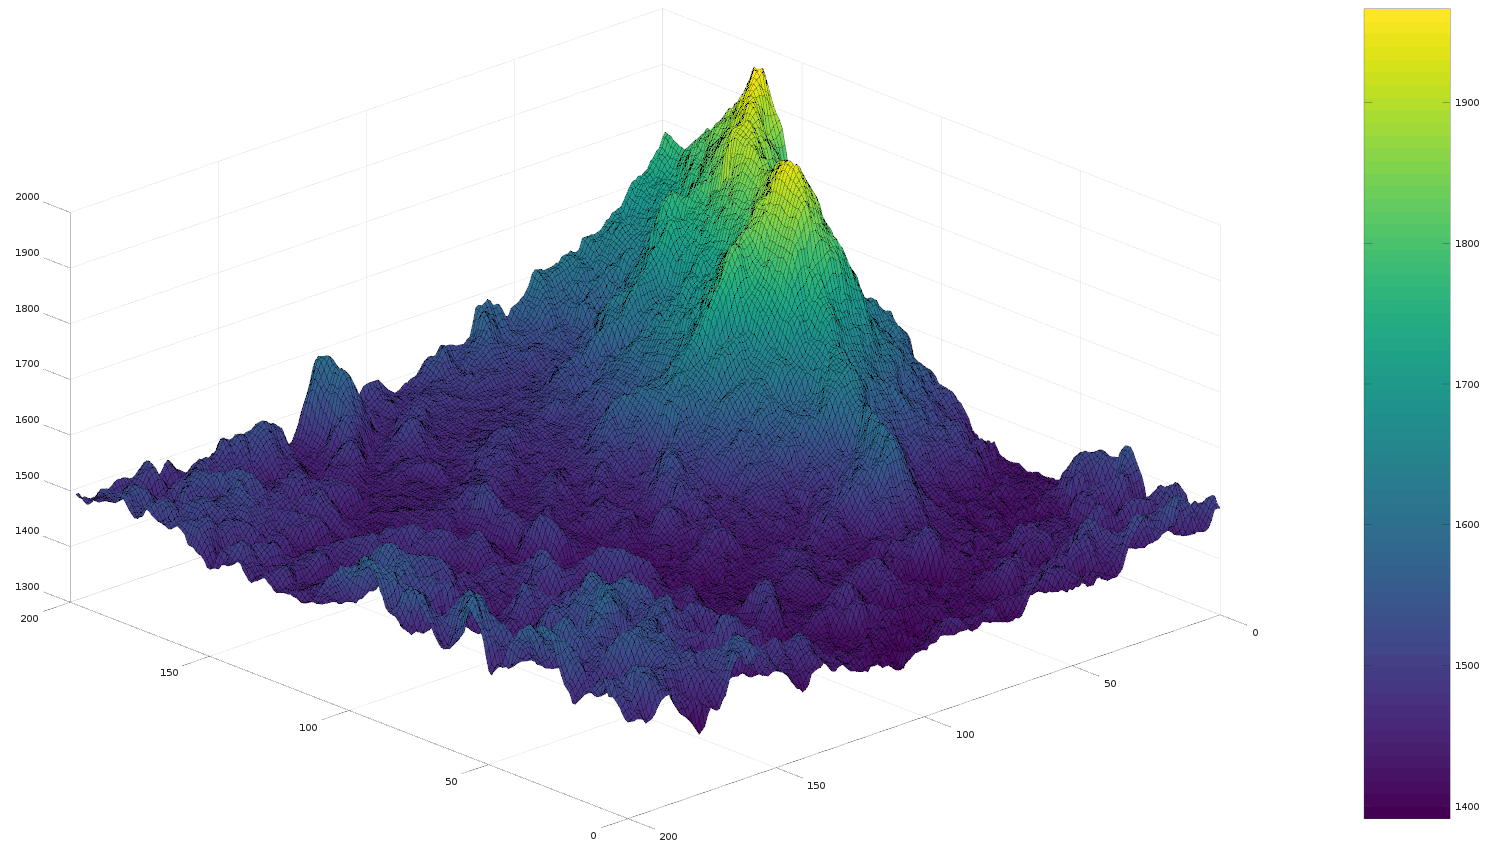
\includegraphics[width=\linewidth]{picture/Selection_038.png}
        \caption{Khu vực T4}
    \end{figure}
\end{frame}

\begin{frame}
    \frametitle{Tham số}
    Tham số chung của các bộ dữ liệu:
    \begin{itemize}
        \item Khu vực cảm  biến A là miền trong không gian 3 chiều với kích thước dài rộng là 200x200, chiều cao và sâu không hạn chế.
        \item Số sensor: 40  
        \item Sensor chôn sâu dưới mặt đất 10m
        \item Số vị trí khả thi đặt relay: 40 
        \item Vị trí đặt relay cao hơn mặt đất 1m
        \item $E_{TX}$ = 50*1e-9
        \item $E_{RX}$ = 50*1e-9
        \item $E_{DA}$ = 10*1e-12
        \item $e_{fs}$ = 10*1e-12
        \item $e_{mp}$ = 0.0013 * 1e-12
    \end{itemize}
\end{frame}

\begin{frame}
    \frametitle{Tham số}
    Tham số giải thuật di truyền:
    \begin{table}[H]
        \begin{tabularx}{\textwidth}{|X|X|}
            \hline
            \multicolumn{1}{|c|}{\textbf{Tham số}} & \multicolumn{1}{c|}{\textbf{Giá trị}}                    \\ \hline
            Số lần chạy 1 bộ dữ liệu  &  20                                                 \\ \hline
            Kích thước quần thể  & 100                                                      \\ \hline
            Số cá thể khởi tạo & 100                                                        \\ \hline
            Số thế hệ & 100                                                                 \\ \hline
            Số thế hệ dừng nếu không cải thiện kết quả & 30                                 \\ \hline
            Tỉ lệ lai ghép & 0.8                                                            \\ \hline
            Tỉ lệ đột biến   & 0.1                                                          \\ \hline
        \end{tabularx}
        \caption{Tham số cài thuật toán GAH}
    \end{table}
\end{frame}

\begin{frame}
    \frametitle{Kịch bản thử nghiệm}
    
    \begin{itemize}
        \item Cài đặt giải bài toán bằng mô hình quy hoạch nguyên nới lỏng.
        \item Chạy mỗi bộ dữ liệu 20 lần.
        \item $\alpha$ = 0.5
    \end{itemize}
\end{frame}

\begin{frame}
    \frametitle{Môi trường thực nghiệm}
    Thông số phần cứng:
    \begin{itemize}
        \item Bộ vi xử lý: Intel core i7-2640M 2.8GHz
        \item RAM: 4GB    
    \end{itemize}
\end{frame}

\begin{frame}
    \frametitle{So sánh kết quả}
    \begin{figure}[h!]
        \centering
        \subfigure{\fbox{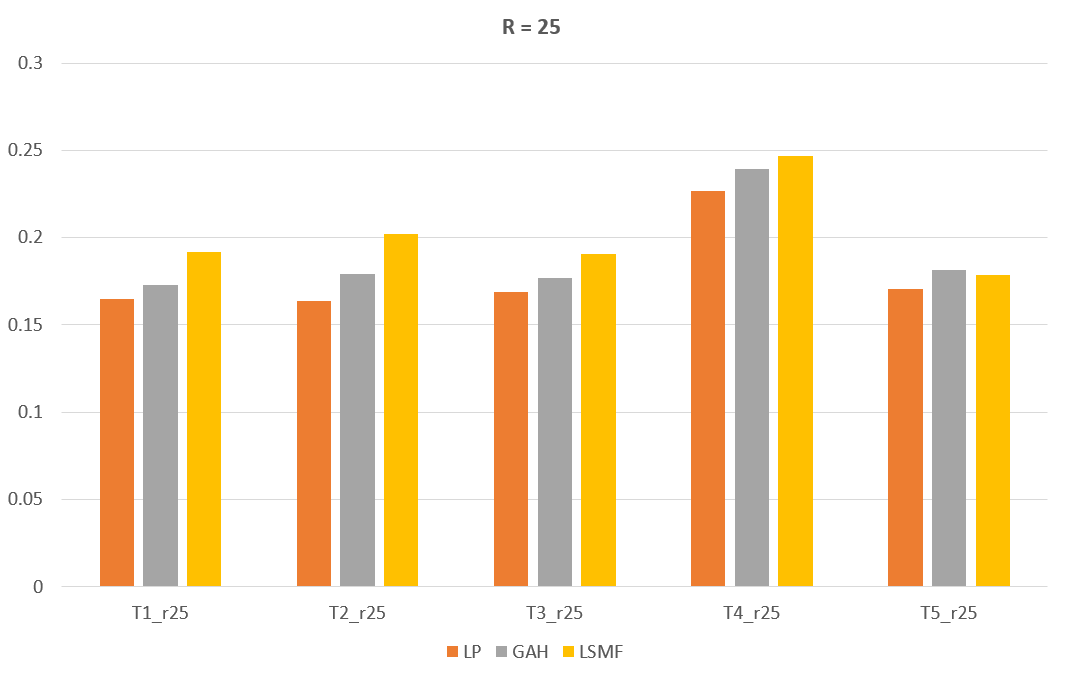
\includegraphics[width=0.4\linewidth]{picture/res_cp_25.png}}}
        \hspace{1cm}
        \subfigure{\fbox{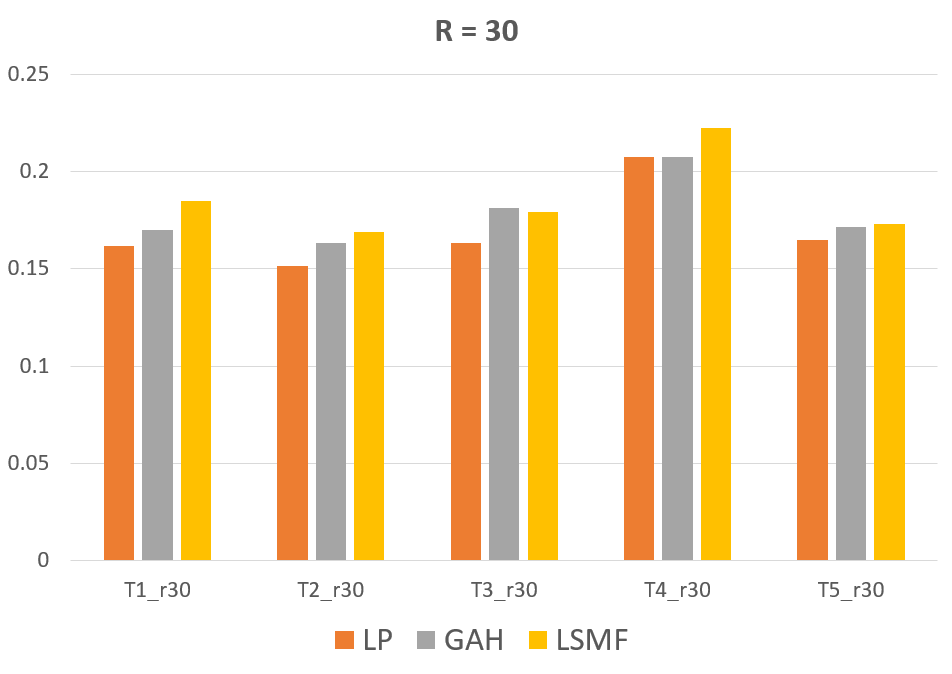
\includegraphics[width=0.4\linewidth]{picture/res_cp_30.png}}}
        \subfigure{\fbox{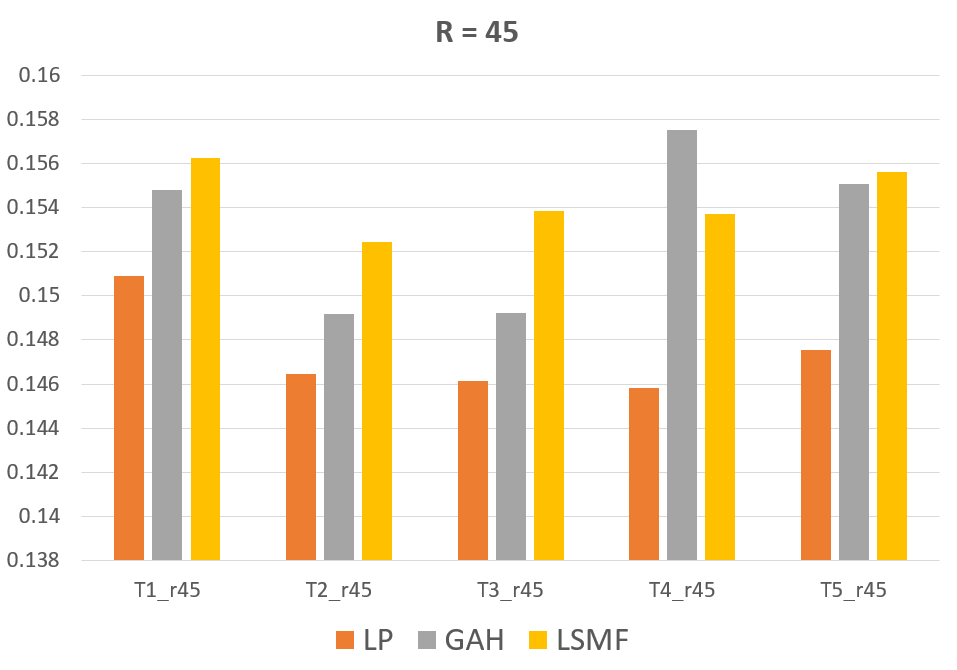
\includegraphics[width=0.4\linewidth]{picture/res_cp_45.png}}}
        \hspace{1cm}
        \subfigure{\fbox{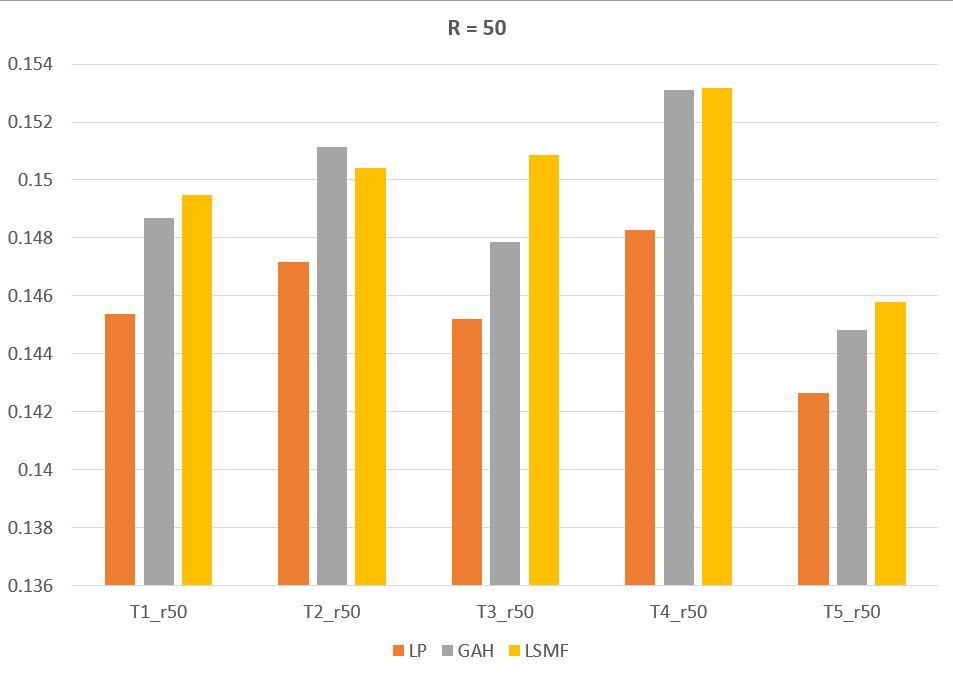
\includegraphics[width=0.4\linewidth]{picture/res_cp_50.png}}}
    \end{figure}
\end{frame}

\begin{frame}
    \frametitle{So sánh thời gian}
    \begin{figure}[h!]
        \centering
        \subfigure{\fbox{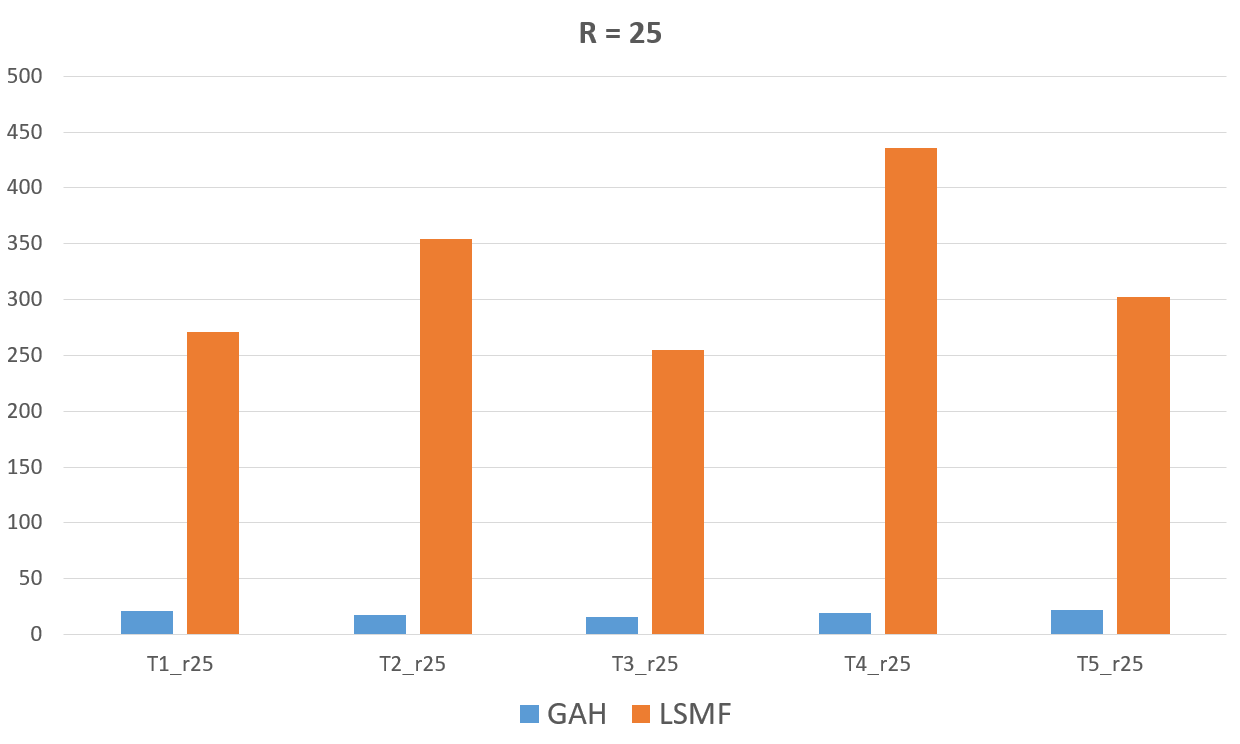
\includegraphics[width=0.4\linewidth]{picture/time_cp_25.png}}}
        \hspace{1cm}
        \subfigure{\fbox{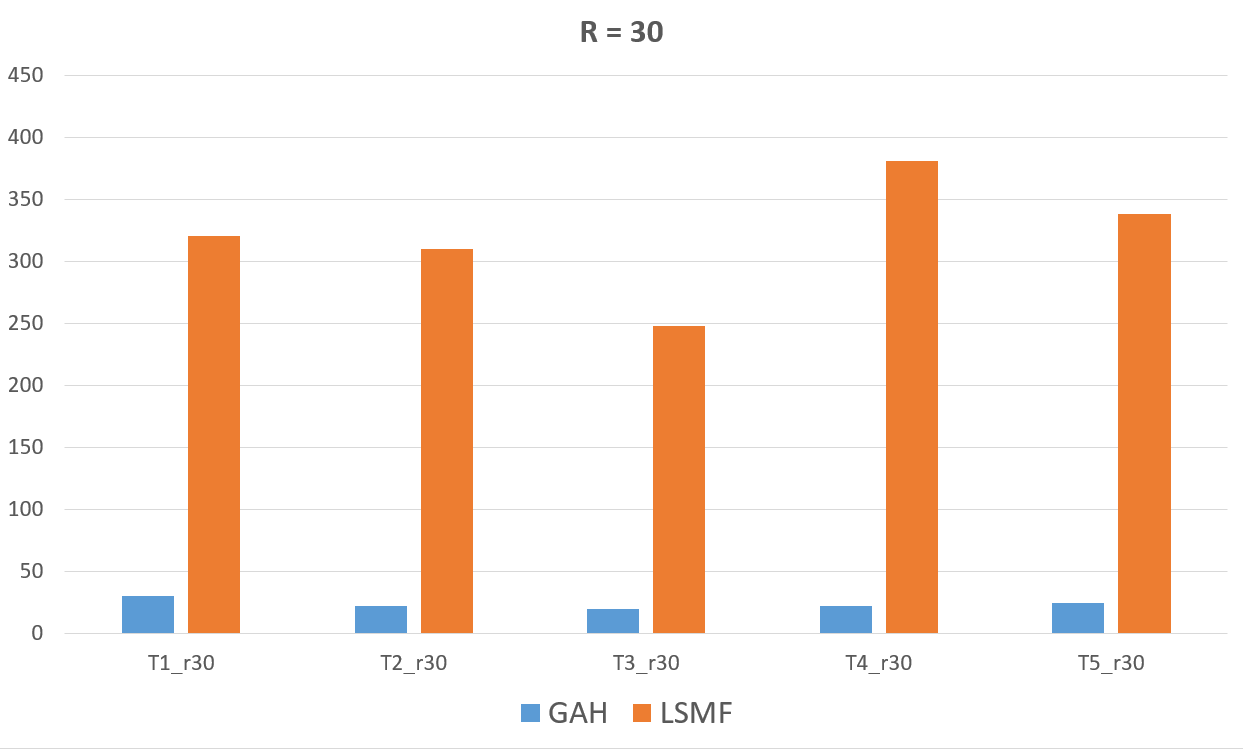
\includegraphics[width=0.4\linewidth]{picture/time_cp_30.png}}}
        \subfigure{\fbox{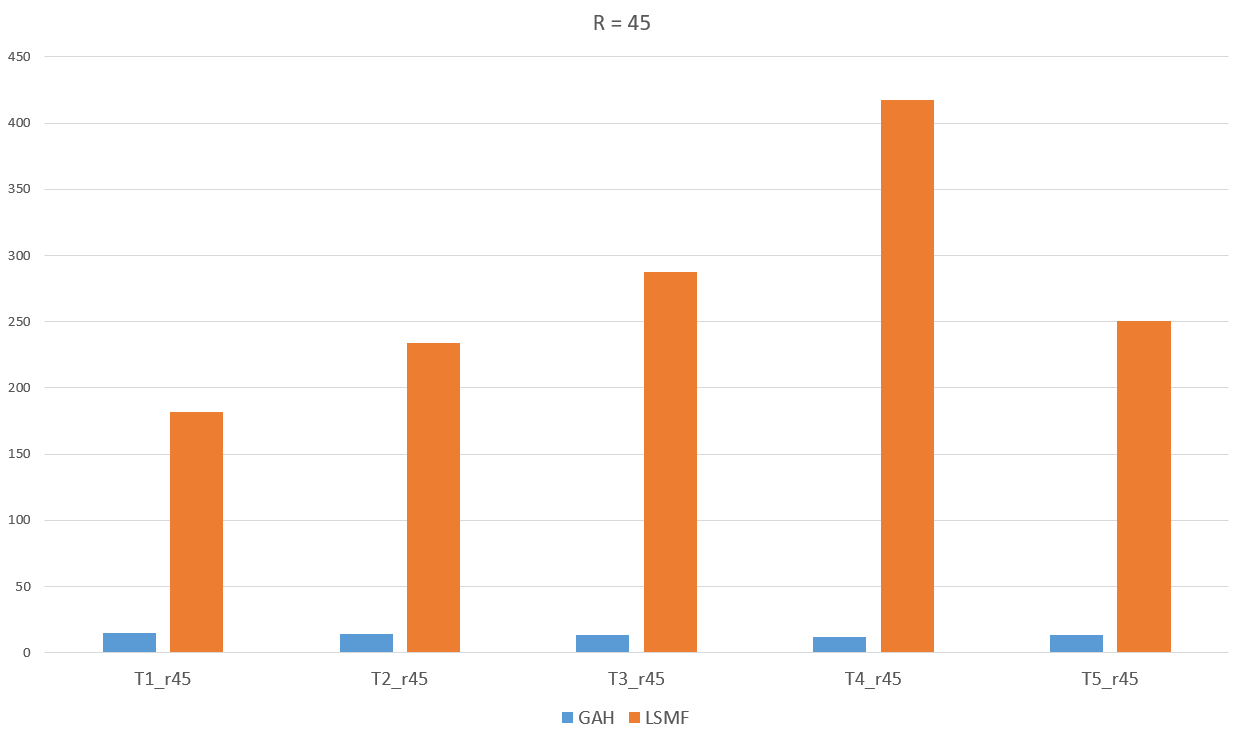
\includegraphics[width=0.4\linewidth]{picture/time_cp_45.png}}}
        \hspace{1cm}
        \subfigure{\fbox{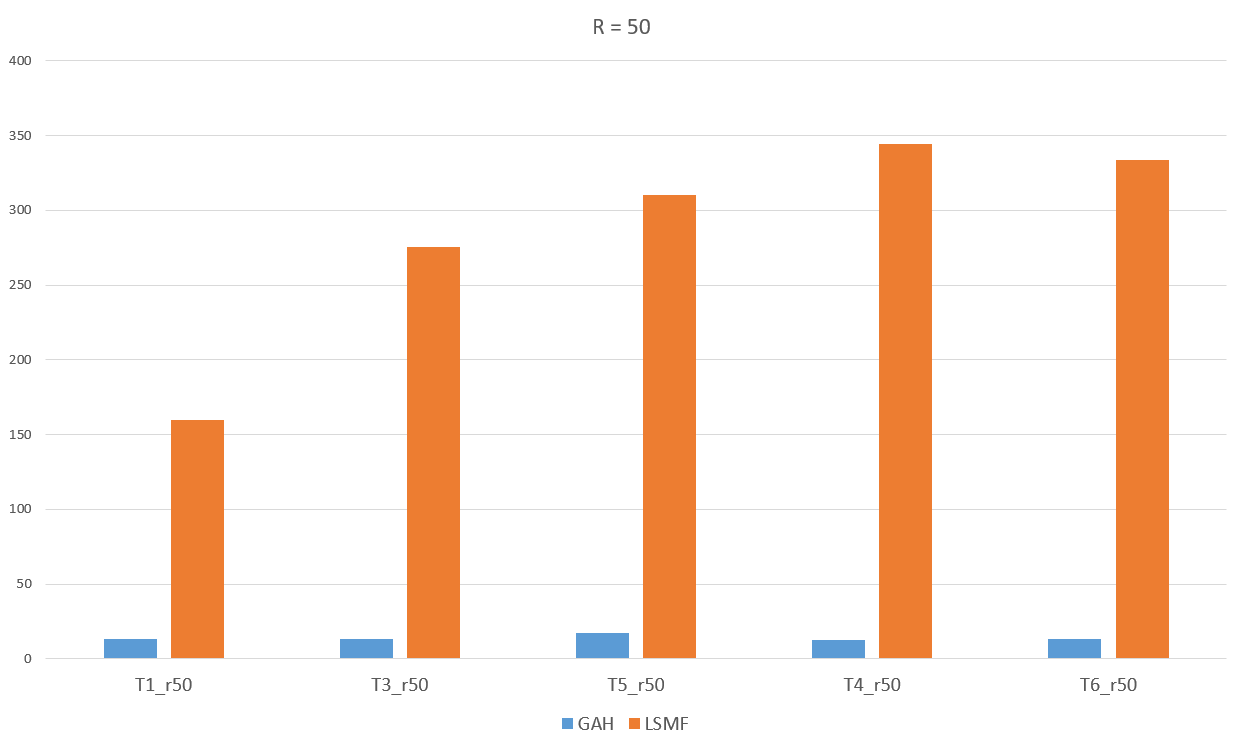
\includegraphics[width=0.4\linewidth]{picture/time_cp_50.png}}}
    \end{figure}
\end{frame}